\documentclass {article}

\usepackage{graphicx}
\usepackage{multicol}
\usepackage{hyperref} 

\usepackage{amsmath}
\begin{document}
	
	
	%
	%Title template { Title } {Workplace } {Name/date }
	%\newcommand{\waterlootitle}[3]{
	%\begin{singlespace}
	% \begin{titlepage}
	%
	%  \begin{center}
	
	% \textbf{\MakeUppercase{ University of Waterloo }} \\
	% \textbf{Faculty of Mathematics}
	
	% \vfill  
	
	%{
	% \large
	%\textsc{\textbf{\textit{#1}}}
	% }
	
	%  \vfill
	
	%#2
	
	%\vfill
	
	%prepared by \\[1em]
	%#3
	
	%\end{center}
	
	%\end{titlepage}
	%\end{singlespace}
	%}
	%
	
	%~\vfill
	\begin{center}
		\Large
		
		\textbf{\MakeUppercase{CSC2521 - Computational Design and Fabrication Fall 2017}}
		\vfill  
		
		{
			\Huge
			\textbf{Assignment 3}
		}
		
		{
			\Large
			\textsc{\textbf{The Finite Element Method}}
		}
		
		\vfill
		Name: Lawson Fulton
		
		Student ID: 998262062
		
		November 3, 2017
	\end{center}
	
	\newpage
	\noindent{\Large \bf Results:}
	\begin{description}
		\item[Basic Functionality]:\\
		
		Uses the finite element method to simulate neo-hookean elasticity on a 2D mesh. 
		
		\begin{figure*}[ht!]
			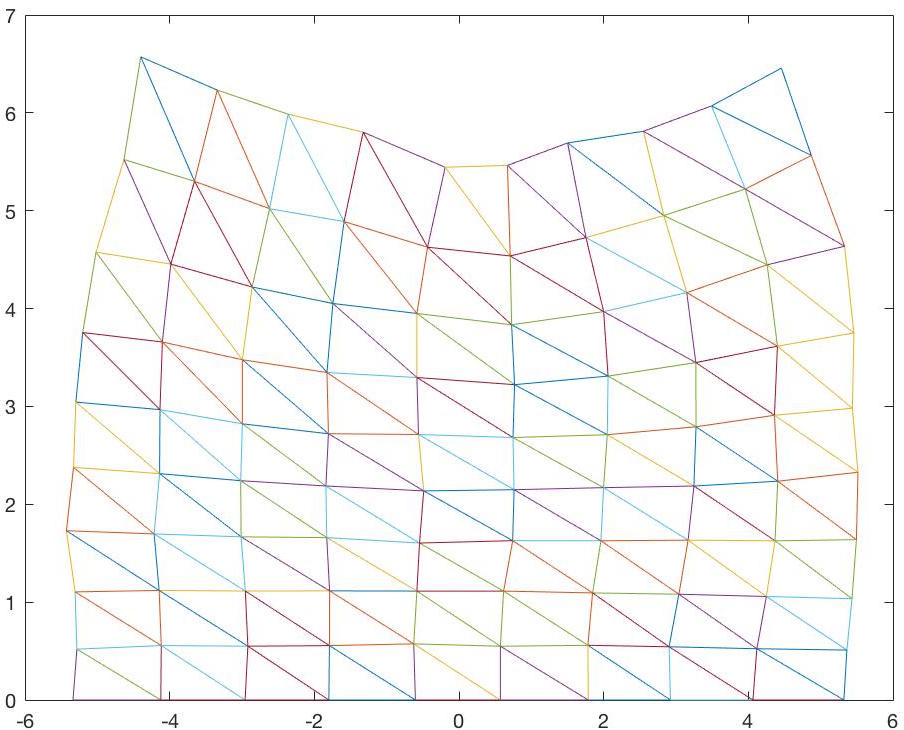
\includegraphics[width=.45\textwidth]{../final_square_10}\hfill
			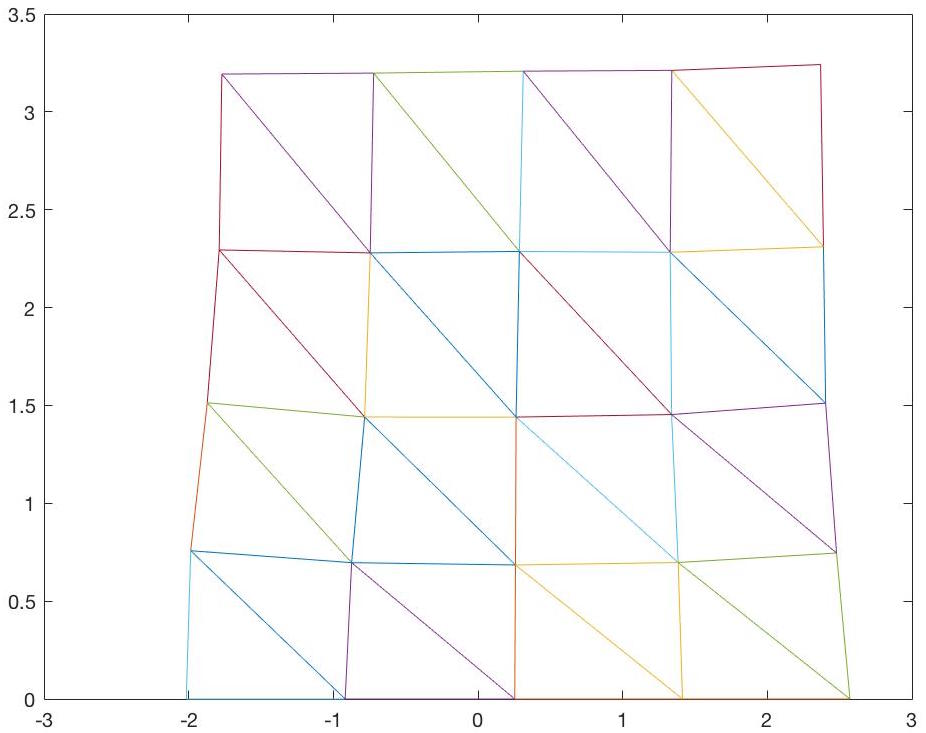
\includegraphics[width=.45\textwidth]{../final_square_5}\hfill
			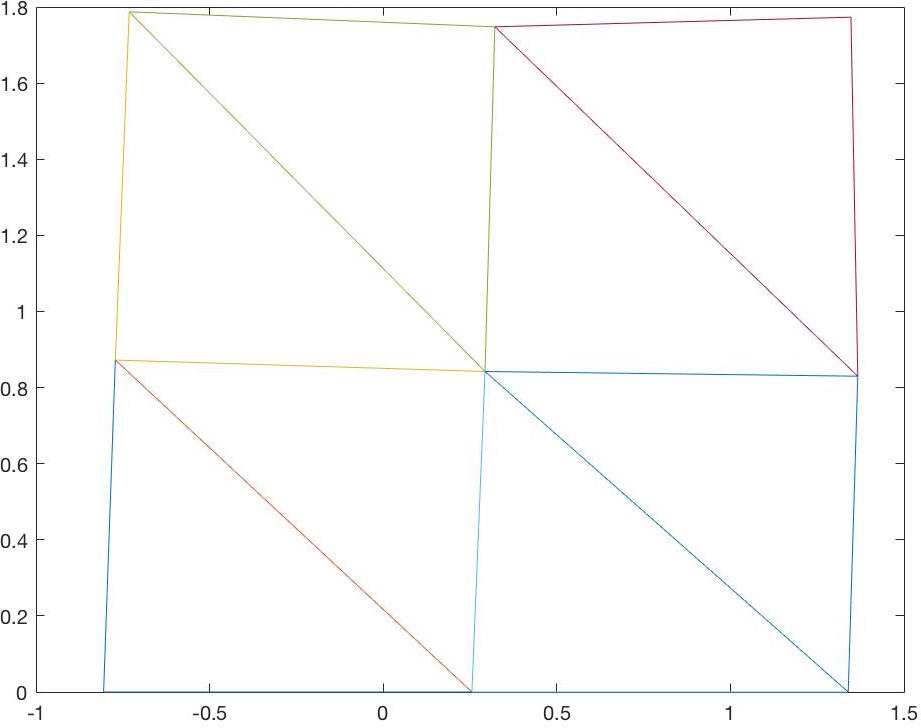
\includegraphics[width=.45\textwidth]{../final_square_3}\hfill
			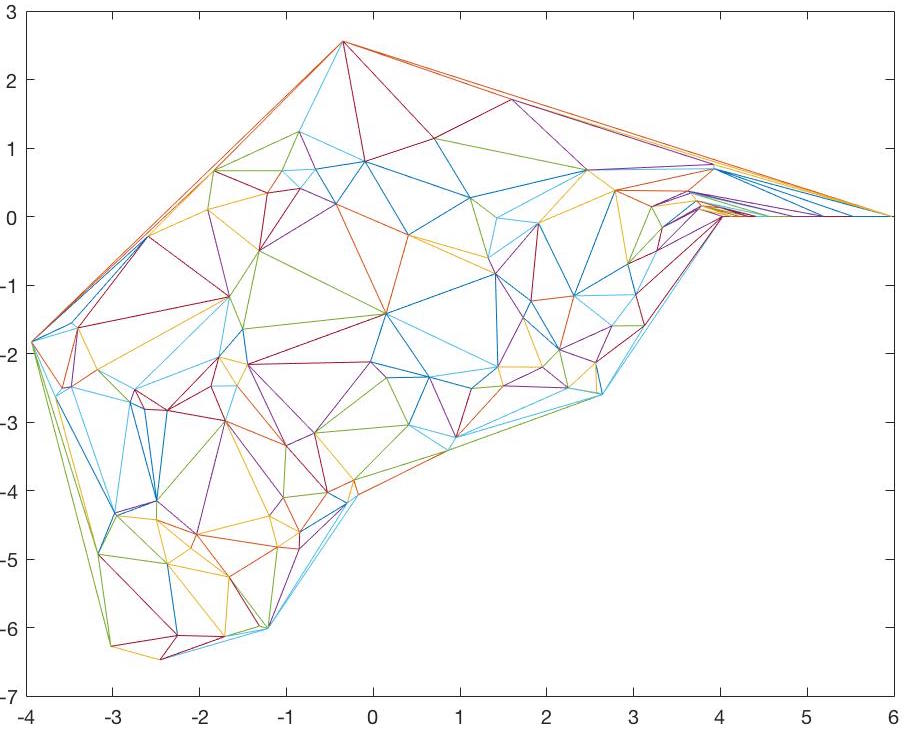
\includegraphics[width=.45\textwidth]{../non-square}\hfill
			\caption{Final frames of 10x10, 5x5, 3x3, and non-square mesh. }
		\end{figure*}
		
		
		
	\end{description}
	
\end{document}
